\subsection{Pourquoi décomposer la table ?}
\paragraph{}{Il y a au début une unique table contenant une vingtaine d'attributs. Pour illustrer la redondance et les dépendances fonctionnelles, cet exemple de tuples ne sera centré que sur quelques attributs pour des raisons de lisibilité}


\begin{figure}
	\label{sch_df}
	\centering
	\ifx\du\undefined
  \newlength{\du}
\fi
\setlength{\du}{15\unitlength}
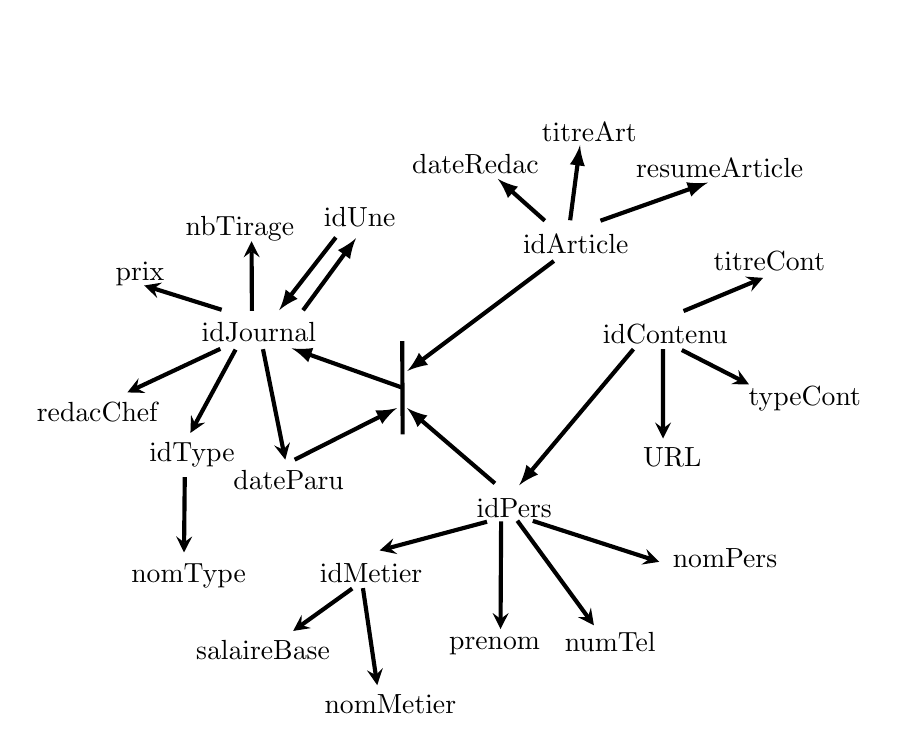
\begin{tikzpicture}[scale=0.9]
\pgftransformxscale{1.000000}
\pgftransformyscale{-1.000000}
\definecolor{dialinecolor}{rgb}{0.000000, 0.000000, 0.000000}
\pgfsetstrokecolor{dialinecolor}
\definecolor{dialinecolor}{rgb}{1.000000, 1.000000, 1.000000}
\pgfsetfillcolor{dialinecolor}
% setfont left to latex
\definecolor{dialinecolor}{rgb}{0.000000, 0.000000, 0.000000}
\pgfsetstrokecolor{dialinecolor}
\node[anchor=west] at (29.900000\du,17.850000\du){idPers};
% setfont left to latex
\definecolor{dialinecolor}{rgb}{0.000000, 0.000000, 0.000000}
\pgfsetstrokecolor{dialinecolor}
\node[anchor=west] at (35.150000\du,19.200000\du){nomPers};
% setfont left to latex
\definecolor{dialinecolor}{rgb}{0.000000, 0.000000, 0.000000}
\pgfsetstrokecolor{dialinecolor}
\node[anchor=west] at (29.163689\du,21.565612\du){prenom};
% setfont left to latex
\definecolor{dialinecolor}{rgb}{0.000000, 0.000000, 0.000000}
\pgfsetstrokecolor{dialinecolor}
\node[anchor=west] at (32.259087\du,21.436290\du){numTel};
% setfont left to latex
\definecolor{dialinecolor}{rgb}{0.000000, 0.000000, 0.000000}
\pgfsetstrokecolor{dialinecolor}
\node[anchor=west] at (25.706125\du,19.600000\du){idMetier};
% setfont left to latex
\definecolor{dialinecolor}{rgb}{0.000000, 0.000000, 0.000000}
\pgfsetstrokecolor{dialinecolor}
\node[anchor=west] at (30.500000\du,21.600000\du){};
% setfont left to latex
\definecolor{dialinecolor}{rgb}{0.000000, 0.000000, 0.000000}
\pgfsetstrokecolor{dialinecolor}
\node[anchor=west] at (25.828978\du,23.102844\du){nomMetier};
\pgfsetlinewidth{0.100000\du}
\pgfsetdash{}{0pt}
\pgfsetdash{}{0pt}
\pgfsetbuttcap
{
\definecolor{dialinecolor}{rgb}{0.000000, 0.000000, 0.000000}
\pgfsetfillcolor{dialinecolor}
% was here!!!
\pgfsetarrowsend{stealth}
\definecolor{dialinecolor}{rgb}{0.000000, 0.000000, 0.000000}
\pgfsetstrokecolor{dialinecolor}
\draw (30.437875\du,18.227601\du)--(27.564463\du,18.995588\du);
}
\pgfsetlinewidth{0.100000\du}
\pgfsetdash{}{0pt}
\pgfsetdash{}{0pt}
\pgfsetbuttcap
{
\definecolor{dialinecolor}{rgb}{0.000000, 0.000000, 0.000000}
\pgfsetfillcolor{dialinecolor}
% was here!!!
\pgfsetarrowsend{stealth}
\definecolor{dialinecolor}{rgb}{0.000000, 0.000000, 0.000000}
\pgfsetstrokecolor{dialinecolor}
\draw (30.816138\du,18.216138\du)--(30.800000\du,21.100000\du);
}
\pgfsetlinewidth{0.100000\du}
\pgfsetdash{}{0pt}
\pgfsetdash{}{0pt}
\pgfsetbuttcap
{
\definecolor{dialinecolor}{rgb}{0.000000, 0.000000, 0.000000}
\pgfsetfillcolor{dialinecolor}
% was here!!!
\pgfsetarrowsend{stealth}
\definecolor{dialinecolor}{rgb}{0.000000, 0.000000, 0.000000}
\pgfsetstrokecolor{dialinecolor}
\draw (31.250000\du,18.200000\du)--(33.300000\du,21.000000\du);
}
\pgfsetlinewidth{0.100000\du}
\pgfsetdash{}{0pt}
\pgfsetdash{}{0pt}
\pgfsetbuttcap
{
\definecolor{dialinecolor}{rgb}{0.000000, 0.000000, 0.000000}
\pgfsetfillcolor{dialinecolor}
% was here!!!
\pgfsetarrowsend{stealth}
\definecolor{dialinecolor}{rgb}{0.000000, 0.000000, 0.000000}
\pgfsetstrokecolor{dialinecolor}
\draw (31.664363\du,18.204676\du)--(35.050000\du,19.300000\du);
}
\pgfsetlinewidth{0.100000\du}
\pgfsetdash{}{0pt}
\pgfsetdash{}{0pt}
\pgfsetbuttcap
{
\definecolor{dialinecolor}{rgb}{0.000000, 0.000000, 0.000000}
\pgfsetfillcolor{dialinecolor}
% was here!!!
\pgfsetarrowsend{stealth}
\definecolor{dialinecolor}{rgb}{0.000000, 0.000000, 0.000000}
\pgfsetstrokecolor{dialinecolor}
\draw (27.117425\du,20.004288\du)--(27.500000\du,22.600000\du);
}
% setfont left to latex
\definecolor{dialinecolor}{rgb}{0.000000, 0.000000, 0.000000}
\pgfsetstrokecolor{dialinecolor}
\node[anchor=west] at (22.500000\du,13.150000\du){idJournal};
% setfont left to latex
\definecolor{dialinecolor}{rgb}{0.000000, 0.000000, 0.000000}
\pgfsetstrokecolor{dialinecolor}
\node[anchor=west] at (18.088100\du,15.300000\du){redacChef};
% setfont left to latex
\definecolor{dialinecolor}{rgb}{0.000000, 0.000000, 0.000000}
\pgfsetstrokecolor{dialinecolor}
\node[anchor=west] at (23.348812\du,17.097434\du){dateParu};
% setfont left to latex
\definecolor{dialinecolor}{rgb}{0.000000, 0.000000, 0.000000}
\pgfsetstrokecolor{dialinecolor}
\node[anchor=west] at (21.096837\du,16.438537\du){idType};
% setfont left to latex
\definecolor{dialinecolor}{rgb}{0.000000, 0.000000, 0.000000}
\pgfsetstrokecolor{dialinecolor}
\node[anchor=west] at (20.198549\du,11.592687\du){prix};
% setfont left to latex
\definecolor{dialinecolor}{rgb}{0.000000, 0.000000, 0.000000}
\pgfsetstrokecolor{dialinecolor}
\node[anchor=west] at (22.069695\du,10.376113\du){nbTirage};
\pgfsetlinewidth{0.100000\du}
\pgfsetdash{}{0pt}
\pgfsetdash{}{0pt}
\pgfsetbuttcap
{
\definecolor{dialinecolor}{rgb}{0.000000, 0.000000, 0.000000}
\pgfsetfillcolor{dialinecolor}
% was here!!!
\pgfsetarrowsend{stealth}
\definecolor{dialinecolor}{rgb}{0.000000, 0.000000, 0.000000}
\pgfsetstrokecolor{dialinecolor}
\draw (23.300000\du,13.600000\du)--(20.812463\du,14.765925\du);
}
\pgfsetlinewidth{0.100000\du}
\pgfsetdash{}{0pt}
\pgfsetdash{}{0pt}
\pgfsetbuttcap
{
\definecolor{dialinecolor}{rgb}{0.000000, 0.000000, 0.000000}
\pgfsetfillcolor{dialinecolor}
% was here!!!
\pgfsetarrowsend{stealth}
\definecolor{dialinecolor}{rgb}{0.000000, 0.000000, 0.000000}
\pgfsetstrokecolor{dialinecolor}
\draw (23.708460\du,13.619674\du)--(22.500000\du,15.850000\du);
}
\pgfsetlinewidth{0.100000\du}
\pgfsetdash{}{0pt}
\pgfsetdash{}{0pt}
\pgfsetbuttcap
{
\definecolor{dialinecolor}{rgb}{0.000000, 0.000000, 0.000000}
\pgfsetfillcolor{dialinecolor}
% was here!!!
\pgfsetarrowsend{stealth}
\definecolor{dialinecolor}{rgb}{0.000000, 0.000000, 0.000000}
\pgfsetstrokecolor{dialinecolor}
\draw (24.442061\du,13.608212\du)--(25.038323\du,16.565538\du);
}
\pgfsetlinewidth{0.100000\du}
\pgfsetdash{}{0pt}
\pgfsetdash{}{0pt}
\pgfsetbuttcap
{
\definecolor{dialinecolor}{rgb}{0.000000, 0.000000, 0.000000}
\pgfsetfillcolor{dialinecolor}
% was here!!!
\pgfsetarrowsend{stealth}
\definecolor{dialinecolor}{rgb}{0.000000, 0.000000, 0.000000}
\pgfsetstrokecolor{dialinecolor}
\draw (22.348439\du,17.035500\du)--(22.327700\du,19.050000\du);
}
\pgfsetlinewidth{0.100000\du}
\pgfsetdash{}{0pt}
\pgfsetdash{}{0pt}
\pgfsetbuttcap
{
\definecolor{dialinecolor}{rgb}{0.000000, 0.000000, 0.000000}
\pgfsetfillcolor{dialinecolor}
% was here!!!
\pgfsetarrowsend{stealth}
\definecolor{dialinecolor}{rgb}{0.000000, 0.000000, 0.000000}
\pgfsetstrokecolor{dialinecolor}
\draw (23.335575\du,12.554150\du)--(21.263275\du,11.904150\du);
}
\pgfsetlinewidth{0.100000\du}
\pgfsetdash{}{0pt}
\pgfsetdash{}{0pt}
\pgfsetbuttcap
{
\definecolor{dialinecolor}{rgb}{0.000000, 0.000000, 0.000000}
\pgfsetfillcolor{dialinecolor}
% was here!!!
\pgfsetarrowsend{stealth}
\definecolor{dialinecolor}{rgb}{0.000000, 0.000000, 0.000000}
\pgfsetstrokecolor{dialinecolor}
\draw (24.145850\du,12.581225\du)--(24.135338\du,10.719661\du);
}
% setfont left to latex
\definecolor{dialinecolor}{rgb}{0.000000, 0.000000, 0.000000}
\pgfsetstrokecolor{dialinecolor}
\node[anchor=west] at (31.100000\du,10.800000\du){idArticle};
% setfont left to latex
\definecolor{dialinecolor}{rgb}{0.000000, 0.000000, 0.000000}
\pgfsetstrokecolor{dialinecolor}
\node[anchor=west] at (28.400000\du,5.250000\du){};
% setfont left to latex
\definecolor{dialinecolor}{rgb}{0.000000, 0.000000, 0.000000}
\pgfsetstrokecolor{dialinecolor}
\node[anchor=west] at (31.605687\du,7.800000\du){titreArt};
% setfont left to latex
\definecolor{dialinecolor}{rgb}{0.000000, 0.000000, 0.000000}
\pgfsetstrokecolor{dialinecolor}
\node[anchor=west] at (28.131821\du,8.650000\du){dateRedac};
% setfont left to latex
\definecolor{dialinecolor}{rgb}{0.000000, 0.000000, 0.000000}
\pgfsetstrokecolor{dialinecolor}
\node[anchor=west] at (33.239777\du,13.200000\du){idContenu};
% setfont left to latex
\definecolor{dialinecolor}{rgb}{0.000000, 0.000000, 0.000000}
\pgfsetstrokecolor{dialinecolor}
\node[anchor=west] at (36.200000\du,11.250000\du){titreCont};
% setfont left to latex
\definecolor{dialinecolor}{rgb}{0.000000, 0.000000, 0.000000}
\pgfsetstrokecolor{dialinecolor}
\node[anchor=west] at (34.313643\du,16.500000\du){URL};
% setfont left to latex
\definecolor{dialinecolor}{rgb}{0.000000, 0.000000, 0.000000}
\pgfsetstrokecolor{dialinecolor}
\node[anchor=west] at (37.139777\du,14.936933\du){typeCont};
\pgfsetlinewidth{0.100000\du}
\pgfsetdash{}{0pt}
\pgfsetdash{}{0pt}
\pgfsetbuttcap
{
\definecolor{dialinecolor}{rgb}{0.000000, 0.000000, 0.000000}
\pgfsetfillcolor{dialinecolor}
% was here!!!
\pgfsetarrowsend{stealth}
\definecolor{dialinecolor}{rgb}{0.000000, 0.000000, 0.000000}
\pgfsetstrokecolor{dialinecolor}
\draw (35.699164\du,12.588049\du)--(37.827700\du,11.700000\du);
}
\pgfsetlinewidth{0.100000\du}
\pgfsetdash{}{0pt}
\pgfsetdash{}{0pt}
\pgfsetbuttcap
{
\definecolor{dialinecolor}{rgb}{0.000000, 0.000000, 0.000000}
\pgfsetfillcolor{dialinecolor}
% was here!!!
\pgfsetarrowsend{stealth}
\definecolor{dialinecolor}{rgb}{0.000000, 0.000000, 0.000000}
\pgfsetstrokecolor{dialinecolor}
\draw (35.148964\du,13.608212\du)--(35.150000\du,16.000000\du);
}
\pgfsetlinewidth{0.100000\du}
\pgfsetdash{}{0pt}
\pgfsetdash{}{0pt}
\pgfsetbuttcap
{
\definecolor{dialinecolor}{rgb}{0.000000, 0.000000, 0.000000}
\pgfsetfillcolor{dialinecolor}
% was here!!!
\pgfsetarrowsend{stealth}
\definecolor{dialinecolor}{rgb}{0.000000, 0.000000, 0.000000}
\pgfsetstrokecolor{dialinecolor}
\draw (35.653314\du,13.631137\du)--(37.450000\du,14.550000\du);
}
% setfont left to latex
\definecolor{dialinecolor}{rgb}{0.000000, 0.000000, 0.000000}
\pgfsetstrokecolor{dialinecolor}
\node[anchor=west] at (22.350000\du,21.665911\du){salaireBase};
\pgfsetlinewidth{0.100000\du}
\pgfsetdash{}{0pt}
\pgfsetdash{}{0pt}
\pgfsetbuttcap
{
\definecolor{dialinecolor}{rgb}{0.000000, 0.000000, 0.000000}
\pgfsetfillcolor{dialinecolor}
% was here!!!
\pgfsetarrowsend{stealth}
\definecolor{dialinecolor}{rgb}{0.000000, 0.000000, 0.000000}
\pgfsetstrokecolor{dialinecolor}
\draw (26.830862\du,20.015751\du)--(25.250000\du,21.150000\du);
}
\pgfsetlinewidth{0.100000\du}
\pgfsetdash{}{0pt}
\pgfsetdash{}{0pt}
\pgfsetbuttcap
{
\definecolor{dialinecolor}{rgb}{0.000000, 0.000000, 0.000000}
\pgfsetfillcolor{dialinecolor}
% was here!!!
\pgfsetarrowsend{latex}
\definecolor{dialinecolor}{rgb}{0.000000, 0.000000, 0.000000}
\pgfsetstrokecolor{dialinecolor}
\draw (34.358051\du,13.608212\du)--(31.300000\du,17.250000\du);
}
\pgfsetlinewidth{0.100000\du}
\pgfsetdash{}{0pt}
\pgfsetdash{}{0pt}
\pgfsetbuttcap
{
\definecolor{dialinecolor}{rgb}{0.000000, 0.000000, 0.000000}
\pgfsetfillcolor{dialinecolor}
% was here!!!
\pgfsetarrowsend{latex}
\definecolor{dialinecolor}{rgb}{0.000000, 0.000000, 0.000000}
\pgfsetstrokecolor{dialinecolor}
\draw (30.650000\du,17.200000\du)--(28.298990\du,15.185069\du);
}
\pgfsetlinewidth{0.100000\du}
\pgfsetdash{}{0pt}
\pgfsetdash{}{0pt}
\pgfsetbuttcap
{
\definecolor{dialinecolor}{rgb}{0.000000, 0.000000, 0.000000}
\pgfsetfillcolor{dialinecolor}
% was here!!!
\pgfsetarrowsend{latex}
\definecolor{dialinecolor}{rgb}{0.000000, 0.000000, 0.000000}
\pgfsetstrokecolor{dialinecolor}
\draw (32.227700\du,11.250000\du)--(28.304924\du,14.192800\du);
}
\pgfsetlinewidth{0.100000\du}
\pgfsetdash{}{0pt}
\pgfsetdash{}{0pt}
\pgfsetbuttcap
{
\definecolor{dialinecolor}{rgb}{0.000000, 0.000000, 0.000000}
\pgfsetfillcolor{dialinecolor}
% was here!!!
\definecolor{dialinecolor}{rgb}{0.000000, 0.000000, 0.000000}
\pgfsetstrokecolor{dialinecolor}
\draw (28.169049\du,13.390424\du)--(28.180511\du,15.889250\du);
}
% setfont left to latex
\definecolor{dialinecolor}{rgb}{0.000000, 0.000000, 0.000000}
\pgfsetstrokecolor{dialinecolor}
\node[anchor=west] at (20.614633\du,19.665911\du){nomType};
\pgfsetlinewidth{0.100000\du}
\pgfsetdash{}{0pt}
\pgfsetdash{}{0pt}
\pgfsetbuttcap
{
\definecolor{dialinecolor}{rgb}{0.000000, 0.000000, 0.000000}
\pgfsetfillcolor{dialinecolor}
% was here!!!
\pgfsetarrowsend{latex}
\definecolor{dialinecolor}{rgb}{0.000000, 0.000000, 0.000000}
\pgfsetstrokecolor{dialinecolor}
\draw (25.290499\du,16.565538\du)--(28.025700\du,15.185069\du);
}
\pgfsetlinewidth{0.100000\du}
\pgfsetdash{}{0pt}
\pgfsetdash{}{0pt}
\pgfsetbuttcap
{
\definecolor{dialinecolor}{rgb}{0.000000, 0.000000, 0.000000}
\pgfsetfillcolor{dialinecolor}
% was here!!!
\pgfsetarrowsend{latex}
\definecolor{dialinecolor}{rgb}{0.000000, 0.000000, 0.000000}
\pgfsetstrokecolor{dialinecolor}
\draw (28.174780\du,14.639837\du)--(25.210048\du,13.585287\du);
}
% setfont left to latex
\definecolor{dialinecolor}{rgb}{0.000000, 0.000000, 0.000000}
\pgfsetstrokecolor{dialinecolor}
\node[anchor=west] at (34.127700\du,8.750000\du){resumeArticle};
\pgfsetlinewidth{0.100000\du}
\pgfsetdash{}{0pt}
\pgfsetdash{}{0pt}
\pgfsetbuttcap
{
\definecolor{dialinecolor}{rgb}{0.000000, 0.000000, 0.000000}
\pgfsetfillcolor{dialinecolor}
% was here!!!
\pgfsetarrowsend{latex}
\definecolor{dialinecolor}{rgb}{0.000000, 0.000000, 0.000000}
\pgfsetstrokecolor{dialinecolor}
\draw (31.985313\du,10.169461\du)--(30.727700\du,9.050000\du);
}
\pgfsetlinewidth{0.100000\du}
\pgfsetdash{}{0pt}
\pgfsetdash{}{0pt}
\pgfsetbuttcap
{
\definecolor{dialinecolor}{rgb}{0.000000, 0.000000, 0.000000}
\pgfsetfillcolor{dialinecolor}
% was here!!!
\pgfsetarrowsend{latex}
\definecolor{dialinecolor}{rgb}{0.000000, 0.000000, 0.000000}
\pgfsetstrokecolor{dialinecolor}
\draw (32.663911\du,10.157999\du)--(32.927700\du,8.150000\du);
}
\pgfsetlinewidth{0.100000\du}
\pgfsetdash{}{0pt}
\pgfsetdash{}{0pt}
\pgfsetbuttcap
{
\definecolor{dialinecolor}{rgb}{0.000000, 0.000000, 0.000000}
\pgfsetfillcolor{dialinecolor}
% was here!!!
\pgfsetarrowsend{latex}
\definecolor{dialinecolor}{rgb}{0.000000, 0.000000, 0.000000}
\pgfsetstrokecolor{dialinecolor}
\draw (33.475438\du,10.169461\du)--(36.350000\du,9.150000\du);
}
\pgfsetlinewidth{0.100000\du}
\pgfsetdash{}{0pt}
\pgfsetdash{}{0pt}
\pgfsetbuttcap
{
\definecolor{dialinecolor}{rgb}{0.000000, 0.000000, 0.000000}
\pgfsetfillcolor{dialinecolor}
% was here!!!
\pgfsetarrowsend{latex}
\definecolor{dialinecolor}{rgb}{0.000000, 0.000000, 0.000000}
\pgfsetstrokecolor{dialinecolor}
\draw (26.392361\du,10.616499\du)--(24.875525\du,12.564625\du);
}
% setfont left to latex
\definecolor{dialinecolor}{rgb}{0.000000, 0.000000, 0.000000}
\pgfsetstrokecolor{dialinecolor}
\node[anchor=west] at (25.772362\du,10.080562\du){idUne};
\pgfsetlinewidth{0.100000\du}
\pgfsetdash{}{0pt}
\pgfsetdash{}{0pt}
\pgfsetbuttcap
{
\definecolor{dialinecolor}{rgb}{0.000000, 0.000000, 0.000000}
\pgfsetfillcolor{dialinecolor}
% was here!!!
\pgfsetarrowsend{latex}
\definecolor{dialinecolor}{rgb}{0.000000, 0.000000, 0.000000}
\pgfsetstrokecolor{dialinecolor}
\draw (25.514962\du,12.567137\du)--(26.931099\du,10.639424\du);
}
% setfont left to latex
\definecolor{dialinecolor}{rgb}{0.000000, 0.000000, 0.000000}
\pgfsetstrokecolor{dialinecolor}
\node[anchor=west] at (29.750000\du,21.450000\du){};
\end{tikzpicture}
	\caption{Schéma des dépendances fonctionnelles de la base de données}
\end{figure} 

\paragraph{Dépendances fonctionnelles}{Les dépendances fonctionnelles de la figure \ref{sch_df} peuvent être retranscrites de la manière suivante.
}
\begin{enumerate}
    \item[(1)] idJournal $\rightarrow$ prix, nbTirage, idUne, idType, redacChef, dateParu
    \item[(2)] idType $\rightarrow$ nomType
    \item[(3)] idUne $\rightarrow$ idJournal
    \item[(4)] idArticle $\rightarrow$ dateRedac, titreArt, resumeArt
    \item[(5)] idContenu $\rightarrow$ URL, titreCont, typeCont
    \item[(6)] idPers $\rightarrow$ nomPers, prenom, numTel, idMetier
    \item[(7)] idMetier $\rightarrow$ salaireBase, nomMetier
    \item[(8)] idArticle, idPers, dateParu $\rightarrow$ idJournal
\end{enumerate}

\paragraph{Clés}{
    De ce schéma, on peut en déduire trois clés $\{idJournal, idArticle, idContenu\}$, $\{idUne, idArticle, idContenu\}$ et $\{dateParu, idContenu, idArticle\}$.
}

\subsection{Algorithme de Bernstein}
\paragraph{}{Une fois nos dépendances fonctionnelles établies, nous commençons par appliquer l'algorithme de Bernstein pour décomposer notre grande table. Tout d'abord, nous déterminons la couverture minimale. On utilisera la clé suivante : \{idJournal, idArticle, idContenu\}. }

\paragraph{}{Les relations (1), (4), (5), (6) et (7) ne sont pas en forme élémentaires, nous les décomposons donc. De plus, à part la relation (8), toutes les autres relations sont qu'un seul attributs à gauche. il n'est donc pas nécessaire de calculer la fermeture de ces attributs. Il est cependant nécessaire de le faire pour la relation (8).}

\paragraph{}{Calcul de la fermeture des attributs en partie gauche de la relation (8) :
\begin{itemize}
\item $idArticle+ = \{dateRedac, titreArt, resumeArticle\}$ 
\item $idPers+ = \{nomPers, numTel, prenom, idMetier, nomMetier, salaireBase\}$
\item $dateParu+ = \{\}$
\end{itemize} }

\paragraph{}{Étant donné qu'aucun élément de chacune des trois fermetures n'apparaît en partie gauche de la relation (8), cette dernière peut être gardée telle quelle.}
\paragraph{}{Au final, la couverture minimale est la suivante :
\begin{enumerate}
    \item[(1.1)] idJournal $\rightarrow$ prix
    \item[(1.2)] idJournal $\rightarrow$ nbTirage
    \item[(1.3)] idJournal $\rightarrow$ idUne
    \item[(1.4)] idJournal $\rightarrow$ idType
    \item[(1.5)] idJournal $\rightarrow$ redacChef
    \item[(1.6)] idJournal $\rightarrow$ dateParu
    \item[(2)] idType $\rightarrow$ nomType
    \item[(3)] idUne $\rightarrow$ idJournal
    \item[(4.1)] idArticle $\rightarrow$ dateRedac
    \item[(4.2)] idArticle $\rightarrow$ titreArt
    \item[(4.3)] idArticle $\rightarrow$ resumeArt
    \item[(5.1)] idContenu $\rightarrow$ URL
    \item[(5.2)] idContenu $\rightarrow$ titreCont
    \item[(5.3)] idContenu $\rightarrow$ typeCont
    \item[(6.1)] idPers $\rightarrow$ nomPers
    \item[(6.2)] idPers $\rightarrow$ prénom
    \item[(6.3)] idPers $\rightarrow$ numTel
    \item[(6.4)] idPers $\rightarrow$ idMetier
    \item[(7.1)] idMetier $\rightarrow$ salaireBase
    \item[(7.2)] idMetier $\rightarrow$ nomMetier
    \item[(8)] idArticle, idPers, dateParu $\rightarrow$ idJournal
\end{enumerate}}

\paragraph{}{Nous créons ensuite nos groupes, en regroupant les dépendances ayant même partie gauche dans chaque groupe :
\begin{enumerate}
    \item[(1)] $DF_1 = \{ (1.1), (1.2), (1.3), (1.4), (1.5), (1.6) \}$
    \item[(2)] $DF_2 = \{ (2) \}$
    \item[(3)] $DF_3 = \{ (3) \}$
    \item[(4)] $DF_4 = \{ (4.1), (4.2), (4.3) \}$
    \item[(5)] $DF_5 = \{ (5.1), (5.2), (5.3) \}$
    \item[(6)] $DF_6 = \{ (6.1), (6.2), (6.3), (6.4) \}$
    \item[(7)] $DF_7 = \{ (7.1), (7.2) \}$
    \item[(8)] $DF_8 = \{ (8) \}$
\end{enumerate}}

\paragraph{}{Puis, nous construisons un schéma $<R_i(U_i),DF_i>$ pour chaque groupe $DF_i$, où $U_i$ est l'ensemble des attributs apparaissant dans $DF_i$ :
\begin{enumerate}
    \item[(1)] $<R_1(idJournal, nbTirage, idUne, idType, redacChef, dateParu), DF_1>$
    \item[(2)] $<R_2(idType, nomType),DF_2>$
    \item[(3)] $<R_3(idUne, idJournal),DF_3>$
    \item[(4)] $<R_4(idArticle, dateRedac, titreArt, resumeArt),DF_4>$
    \item[(5)] $<R_5(idContenu, URL, titreCont, typeCont),DF_5>$
    \item[(6)] $<R_6(idPers, nomPers, prenom, numTel, idMetier),DF_6>$
    \item[(7)] $<R_7(idMetier, salaireBase, nomMetier),DF_7>$
    \item[(8)] $<R_8(idArticle, idPers, dateParu, idJournal),DF_8>$
\end{enumerate}}

\paragraph{}{Pour terminer, comme la clé entière n'est présente dans aucun schéma, on rajoute un dernier schéma de la forme : $<R_9(idJournal, idArticle, idContenu), \{\}>$}

\paragraph{}{Nous obtenons donc, par application de l'algorithme de Bernstein, un ensemble de relations \textit{spi}, \textit{spdf} et en 3ème forme normale.}
 
\subsection{Algorithme de décomposition}
\paragraph{}{
On considère la relation de départ : \\
$R (idJournal, idContenu, idArticle, titreCont, typeCont, URL, dateRedac, \\
titreArt, resumeArticle, idPers, nomPers, numTel, prenom, idMetier,\\ salaireBase, nomMetier, dateParu, idUne, nbTirage, prix, \\
redacChef,  idType, nomType), \\
DF= \{(1),(2),(3),....(8)\}$
}

\paragraph{}{
On décompose la relation avec l'algorithme. Plusieurs résultats sont possibles : dans cette exécution nous avons arbitrairement choisi l'ordre nous permettant de conserver les sous-ensembles les plus proches de la réalité de notre table.
Les tables obtenues sont celles-ci :

$R_1(idMetier, salaireBase, nomMetier), DF_1=\{(7)\}$

$R_{1.1}(idType, nomType), DF_{1.1}=\{(2)\}$

$R_{2.1}(idPers, nomPers, prenom, numTel, idMetier), DF_{2.1}=\{(6)\}$

$R_{3.1}(idContenu, URL, idPers, titreCont, typeCont), DF_{3.1}=\{(5)\}$

$R_{4.1}(idJournal, idUne, nbTirage, prix, redacChef, idType, dateParu), \\DF_{4.1}=\{(41)\}$

$R_{5.1}(idArticle, dateRedac, titreArt, resumeArticle), DF_{5.1}=\{(4)\}$

$R_{5.2}(idJournal, idUne, nbTirage, prix, redacChef, idType, dateParu), \\DF_{5.2}=\{(1)\}$
}
